\section{Introduction}

%1. Current IO structure
% In today's high-performance computing (HPC) systems,
% application's performance is no longer only throttled by computation capability,
% but also perceived I/O rate between
% numerous amount of parallel processor cores and 
% petabyte volume of storage equipments.
% Current IO architects put IO forwarding nodes in charge of performing IO.
% These IO gateways, together with parallel file system (PFS) software (client side),
% sits between internal system networks that serving communication
% between compute nodes and external system networks
% that interconnects storage nodes\cite{Ross:IOSystem}.
% Applications under this architecture can expect to achieve
% 810 GB/s per PFS sustained bandwidth in Trinity's Lustre\cite{TrinitySystem}
% in later 2016, but still far from the target of 60 TB/s
% for extra-scale computing platform\cite{Shalf:HPCCS:2010}.

% %2. Challenge to current IO architecture and burst buffer come to resuce.
% The challenge roots in the missing gap in HPC's memory hierarchy.
% The ratio of IO rate of memory on the compute node to the storage disk
% is 100 to 10,000 cycles\cite{TrinitySystem}.
% Such a gap makes difference because scientific applications on HPC are exposed to
% bursty IO patterns\cite{Carns:MSST:2011, Kim:PDSW:2010},
% resulting from application's
% defensive IO strategy\cite{Latham:CSD:2012, Naik:ICPPW:2009, Dennis:CUG:2009}
% and the needs of subsequent processing of application output.
% 
% 
% %On one hand, applications checkpoint periodically
% %(so that computation could be restarted after system fault)
% %or store intermediate output for subsequent analysis or visualization;
% %on the other hand, pushing data from memory to external,
% %parallel file system is unproductive due to the IO cycle gap.
% %Though this conflict can be fixed by providing higher IO bandwidth capacity,
% %another character of bursty IO pattern introduces another problem,
% %underutilization of storage system.
% %Production applications could generate hundreds of GB to
% %tens of TB data in one IO request with significant idle interval.
% %For example, observed idle interval of write-intensive jobs
% %reported on Intrepid\cite{Liu:MSST:2012},
% %varies from several minutes to 2 hours.
% 
% %3. Very high level intro to burst buffer
% As an alternative storage design, burst buffer\cite{Bent:HBP:2011, Grider:EXA:2010}
% is targeting on fixing the issues caused by bursty IO pattern.
% It fills the gap in memory hierarchy with storage hardware technology
% faster than traditional disks.
% Bursty IO requests could thus be efficiently absorbed and spread out
% into burst buffer nodes.
% Researchers\cite{Liu:MSST:2012} have demonstrated that application perceived IO
% bandwidth are significantly improved on burst buffer enabled system.
% Given its usefulness, we expect user will explicitly request for
% this new resource upon job submission.


%================XY====================
The performance of supercomputers is no longer only throttled by computation capability,
but also perceived I/O rate between
numerous amount of compute nodes and 
petabyte volume of storage equipments.
The IO nodes reside between the compute nodes and external storage, 
serving as IO gateways for the data communication. 
They can deliver 810 GB/s IO performance for applications running on the early-stage Trinity system~\cite{TrinitySystem}, 
but still far from the target of 60 TB/s
for extra-scale computing platform\cite{Shalf:HPCCS:2010}.
%2. Challenge to current IO architecture and burst buffer come to resuce.
The challenge roots in the missing gap in supercomputers' memory hierarchy.
The IO rate ratio of memory to external storage 
is 100 to 10,000 cycles\cite{TrinitySystem}.
Such a gap makes difference because HPC scientific applications are exposed to
bursty IO patterns\cite{Carns:MSST:2011, Kim:PDSW:2010},
resulting from application's
defensive IO strategy\cite{Latham:CSD:2012, Naik:ICPPW:2009, Dennis:CUG:2009}
and the needs of subsequent processing of application output.


%3. Very high level intro to burst buffer
As an alternative storage design, burst buffer\cite{Bent:HBP:2011, Grider:EXA:2010}
is targeting on fixing the issues caused by the bursty IO pattern.
Burst Buffer fills the gap in memory hierarchy with storage hardware technology
faster than traditional disks.
Bursty IO requests could thus be efficiently absorbed and spread out
into burst buffer nodes.
Researchers\cite{Liu:MSST:2012} have demonstrated that application perceived IO
bandwidth are significantly improved on the burst buffer enabled system.
Given its usefulness, we expect user will explicitly request for
this new resource upon job submission.

\begin{figure}[!t]
        \centering
        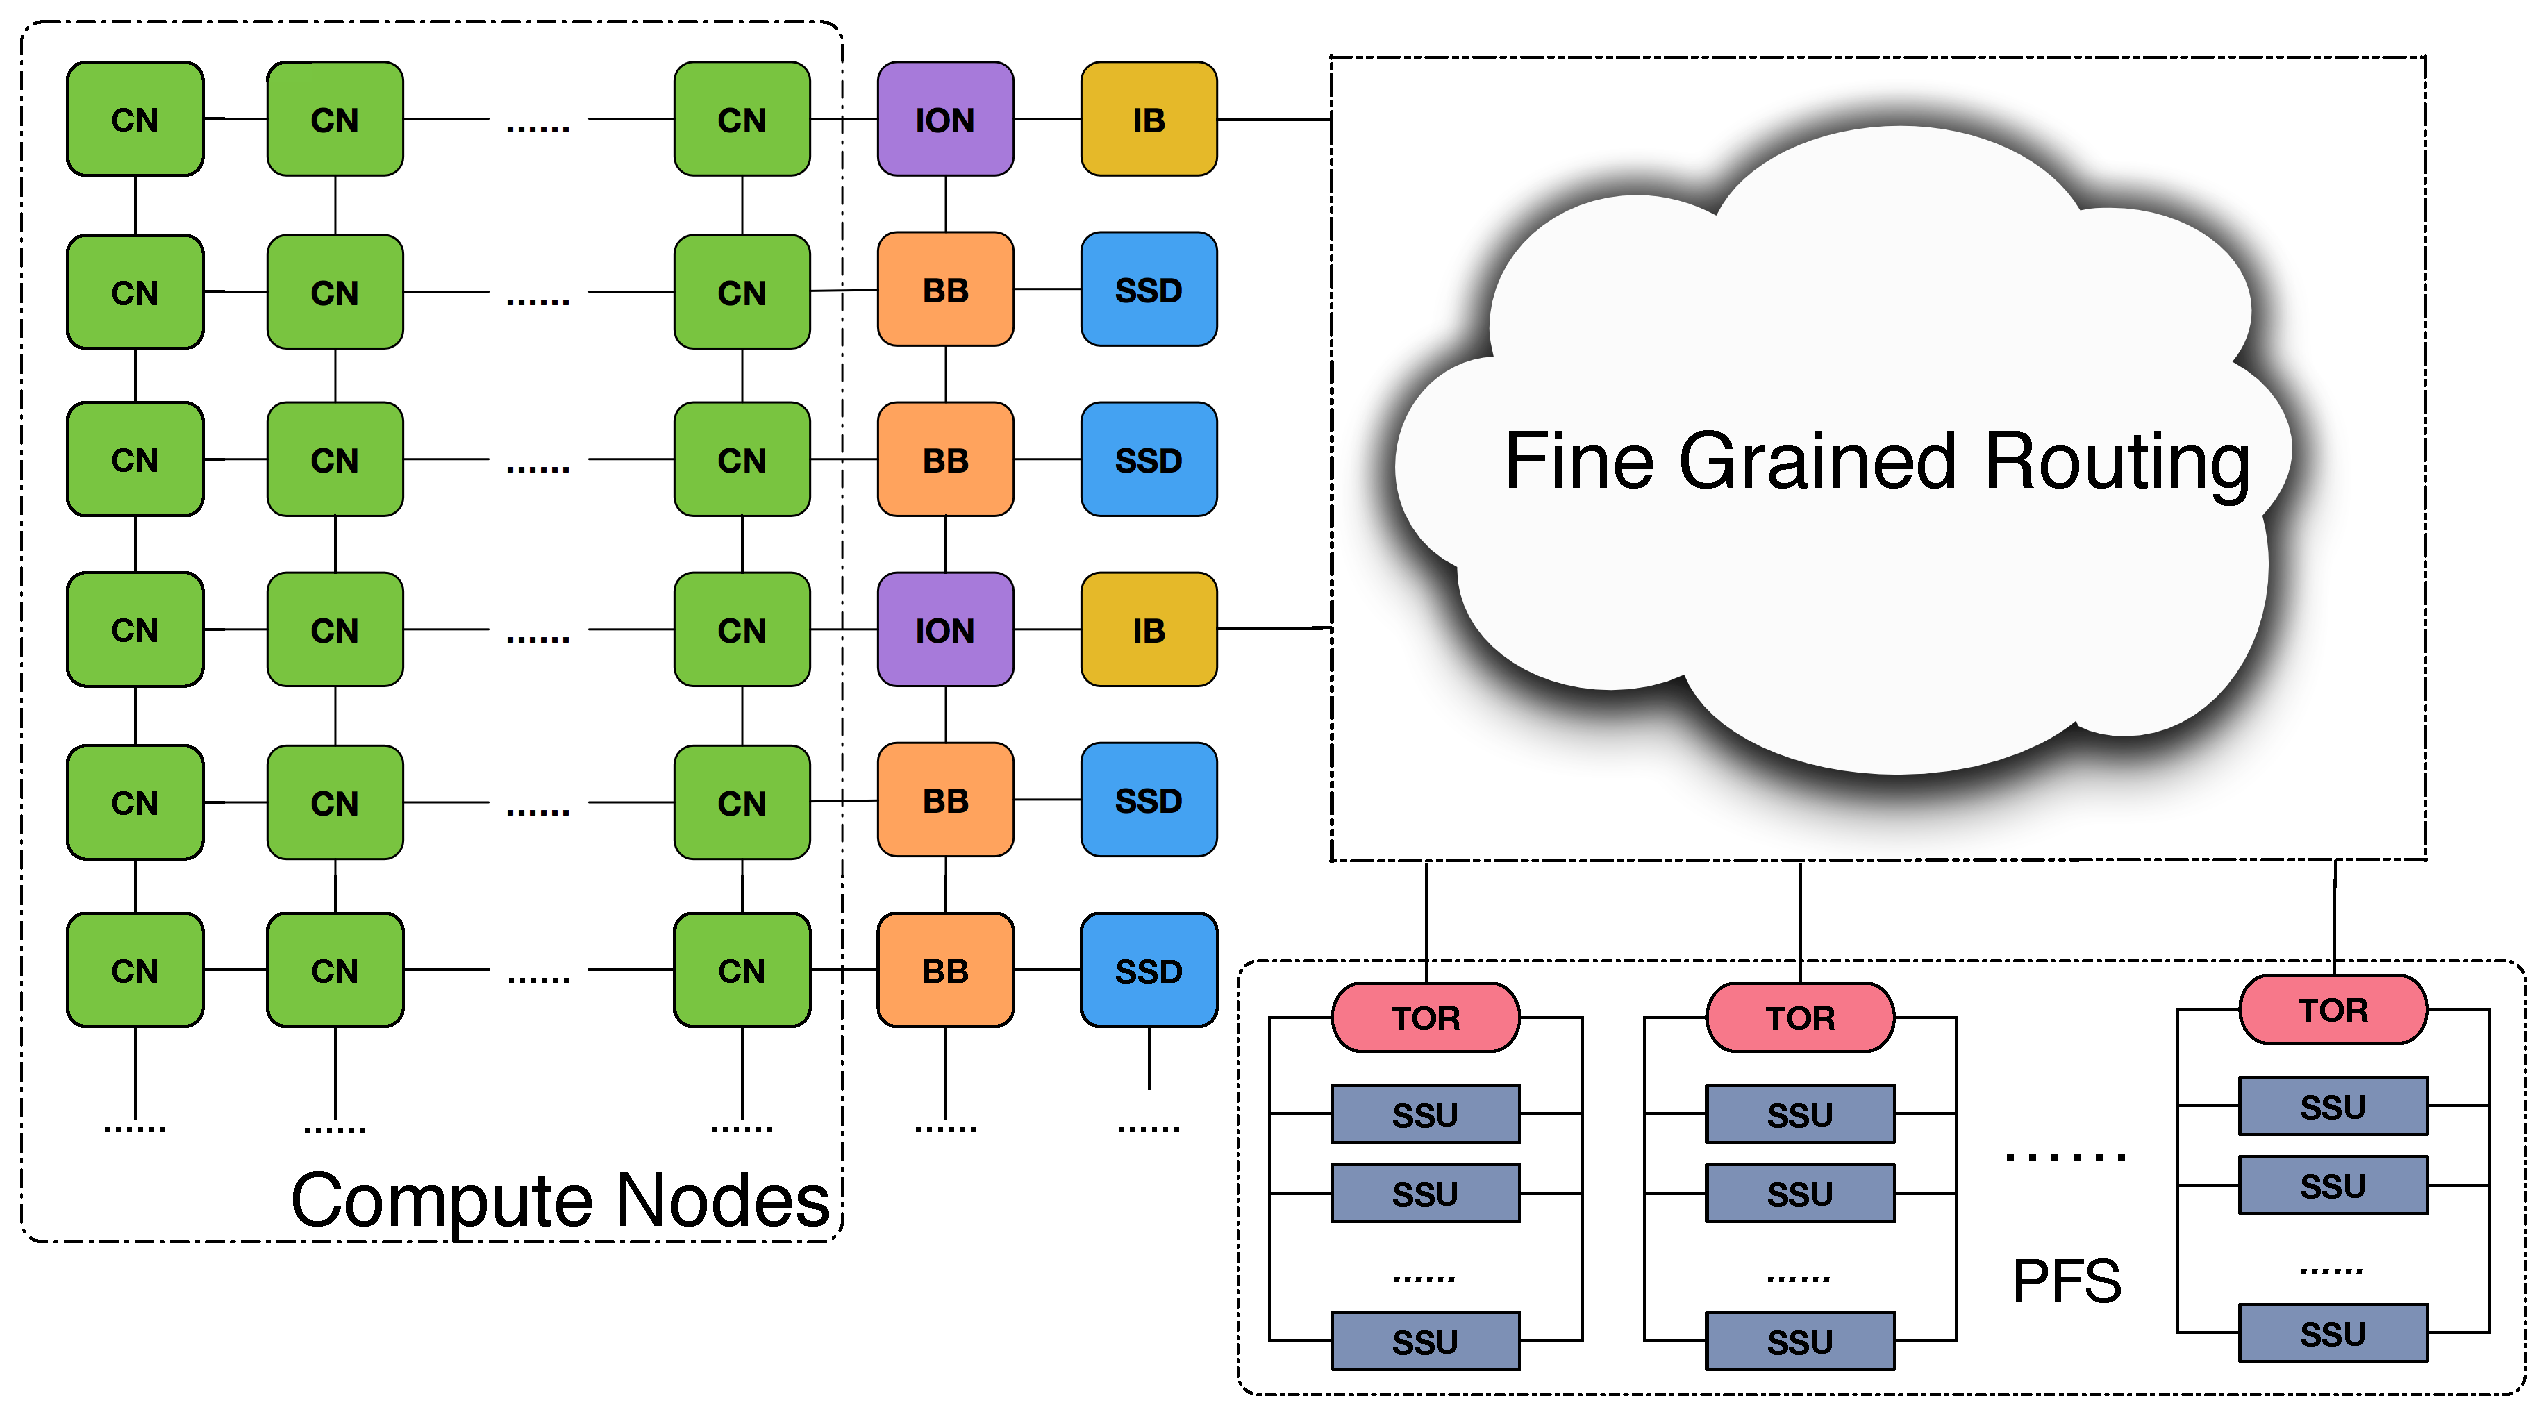
\includegraphics[width= 3.5in]{BBArchitectureShort}
        \caption{Trinity System Overview: A Burst Buffer Enabled Supercomputer}
        \label{Fig:BBArchitecture}
\end{figure}


%===============================================

%4. Our work, a new batch scheduler
% In this paper, we propose Cerberus\footnote{In Greek mythology,
% Cerberus is a monstrous multi-headed dog (3-phase scheduling scheme),
% who guards the gates of the underworld to earth (HPC system),
% preventing the dead (jobs) from leaving (running).},
% a novel batch scheduler for burst buffer enabled HPC systems. 
% We propose a 3-phase model for user job 
% based on two of the most important usage cases of burst buffer: 
% application checkpoint restart and data pre-fetch/cache for stage in/out. 
% The lifetime of user job is divided into \textit{stage in} phase, 
% \textit{running} phase, and \textit{stage-out} phase. 
% Unlike existing batch schedulers that 
% make the one-off scheduling decision for a job upon its submission, 
% Cerberus re-evaluates the job's requirement at each phase 
% and makes the optimal scheduling decisions respectively.

%=============XY=================
In this paper, we propose Cerberus
\footnote{In Greek mythology,
Cerberus is a monstrous 3-headed dog,
who guards the gates of the underworld. In this paper, we personify our 3-phase batch scheduler
in the form of this mythological character.
},
a novel batch scheduler for burst buffer enabled HPC systems. 
We propose a 3-phase model for user job 
based on the most important usage cases of burst buffer: 
application checkpoint restart and staging in/out data. 
The lifetime of user job is divided into \textit{stage in} phase, 
\textit{running} phase, and \textit{stage-out} phase. 
Unlike existing batch schedulers that 
make the one-off scheduling decision for a job upon its submission, 
Cerberus re-evaluates the job's requirement at each phase 
and makes the optimal scheduling decisions respectively.

%5. The advantage of Cerberus.
Both the system and user jobs can benefit from Cerberus 3-phase scheduling.
System responsiveness can be greatly improved and
user jobs suffer less wait time. 
The burst buffer and compute nodes will be released immediately
if the job don't need them in the next phase,
and become available to the following jobs.
As Cerberus takes advantage of the parallelism of jobs in different phases,
system throughput also gets improved.
%6. Summarize our contribution
% Our contributions in this paper are summarized as follows:
% \begin{enumerate}
%         \item %Explore how HPC workload scheduler allocates burst buffer resources.
%                 We propose a 3-phase application model tailored the typical
%                 usage scenarios of burst buffer, that is, checkpoint restart,
%                 data stage in and stage out.
%         \item On the basis of 3-phase job model, we present Cerberus,
%                 a burst buffer aware HPC workload scheduler.
%                 Dividing the lifetime of user application to different phases,
%                 Cerberus conquers the scheduling goal separately.
%         \item We suggest different optimizing goals for each phases.
%                 Though optimal scheduling problem in each phase is NP-hard,
%                 dynamic programming with memorization could give precise solutions
%                 in practice.
%         \item We develop BBSim, a event-driven simulator for scheduling
%                 BB enabled HPC system.
%                 BBSim is motivated by simulating Cerberus
%                 on burst buffer enabled systems but also supports various kind of job schedulers.
%                 %It help us simulate and compare the scheduling results of
%                 %Trinity, a systems with both traditional IO nodes and burst buffer nodes.
% \end{enumerate}
%===========XY==========
Our contributions in this paper are summarized as follows:
\begin{enumerate}
        \item %Explore how HPC workload scheduler allocates burst buffer resources.
                We propose a 3-phase job model tailored the typical
                usage scenarios of burst buffer, that is, checkpoint restart,
                data stage in and stage out.
        \item   We present Cerberus,
                a burst buffer aware batch scheduler for 3-phase modeled jobs.
                Dividing the lifetime of user job to different phases,
                Cerberus can make the optimal scheduling decision 
                for each job separately in each phase.
        \item   We suggest different optimizing goals for each phases.
                Though optimal scheduling problem in each phase is NP-hard,
                dynamic programming could give precise solutions
                in practice.
        \item   We develop BBSim, a event-driven simulator for scheduling
                burst buffer enabled HPC systems.
                BBSim is motivated by simulating Cerberus scheduling 
                3-phase modeled jobs with burst buffer requirement,
                it also supports various kind of batch schedulers.
\end{enumerate}


In the reminder of this paper,
the next section talks about the status quo of burst buffer and
the motivation of our work.
Section~\ref{Sec:Model} begins elaborating the 3-phase model,
after which Cerberus is introduced.
Core events in simulating Cerberus and execution logic of BBSim are
briefly discussed in Section~\ref{Sec:Simulation}.
The details of formulating and solving scheduling problems with
dynamic programming at each job phase are enumerated in Section~\ref{Sec:Scheduler}.
We validate Cerberus by simulating the burst buffer enabled
Trinity supercomputing platform on BBSim (Section~\ref{Sec:Experiments}).
Related works are discussed in Section~\ref{Sec:RelatedWorks}.
We conclude this paper and list possible future works in Section~\ref{Sec:Conclusion}.


\begin{figure}[!htbp]
        \centering
        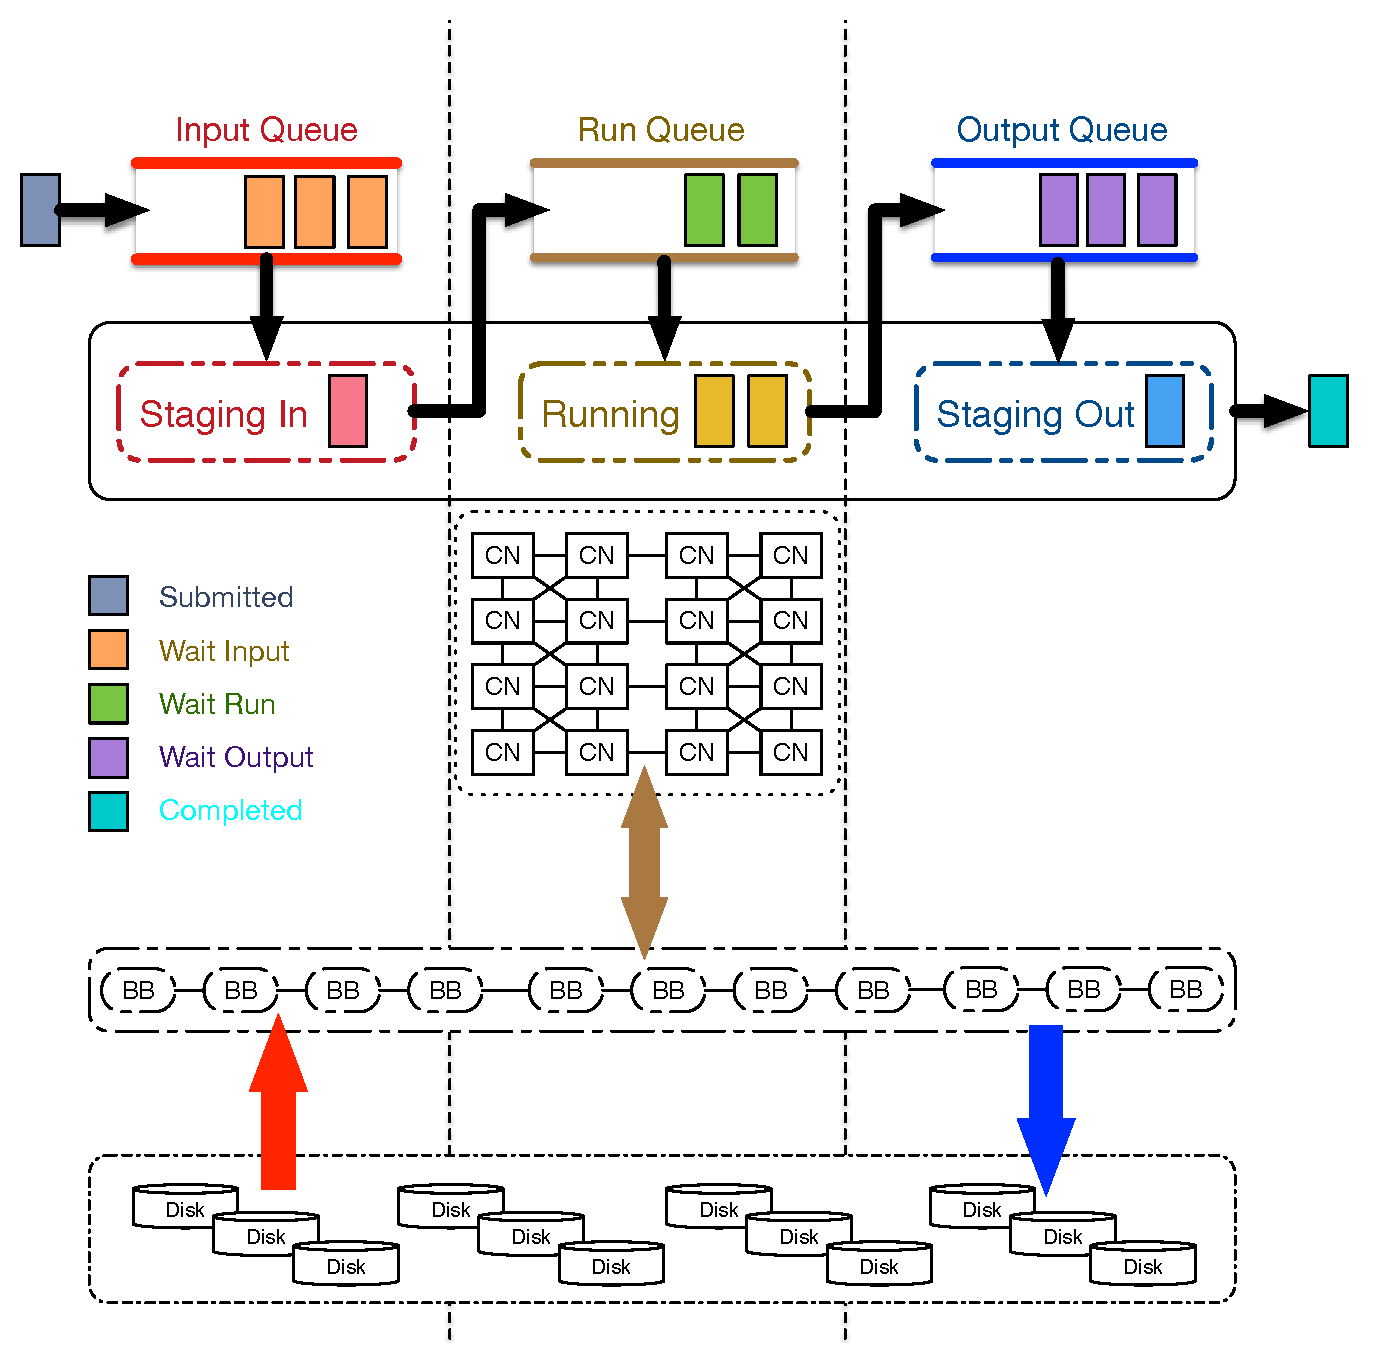
\includegraphics[width=3.6in]{CerberusBBSystem}
        \caption{Scheduling Workflow of Burst Buffer Aware Cerberus}
        \label{Fig:CerberusQueues}
\end{figure}

